\section{User Test Evaluation} % (fold)
\label{sec:User Test Evaluation}
\subsection{Introduction} % (fold)
\label{sub:Introduction}
We conducted user tests with various developers to get feedback on the library.
In total, 13 people participated in this test. All those received a link to a
GitHub repository containing the description of two tasks:
\begin{enumerate}
\item \textbf{Numerical differentiation}: The idea is to use sequences to get
  an approximation as close as possible to the slope of a function |f| at point
  |x|. Lazyness and operations on sequences make this possible.
\item \textbf{Browse JSON files}: In JavaScript you frequently work with JSON
  files provided by some API. This data is often full of holes, which makes it
  difficult to process. JINQ simplifies this task significantly because it
  fills such gaps automatically. 
\end{enumerate}
Both tasks are pleasent use cases of the artifacts of this work.
Chapter~\ref{sec:Examples} describes them in detail.\\
Finally, each participant filled out a questionnaire. This procedure enables
the detection of difficulties and shows where the API still has room for
improvement. 

The findings are based on the questionnaire evaluation and the code of three
participants who handed in their solution. This chapter lists all the
improvements the user test pointed out. In addition, it concludes the general
impression collected by the user test.
Appendix~\ref{chap:app_user_test_results} contains all the user test questions
and their answers.
% subsection Introduction (end)
\subsection{Findings for the Sequence library} % (fold)
\label{sub:Findings for the sequence library}
\subsubsection{General findings and improvements} % (fold)
\label{subsub:Numerical Differentiation Sequence library}
We decided to include following findings in the Sequence library:
\begin{itemize}
  \item \textbf{Renaming untilFunction}: Creating sequences using the sequence
    constructor worked well for everyone. The meaning of the parameters was
    clear to all. (\ref{sub:ut_q3}) However, a suggestion for a meaningful
    optimization from two participants was to rename the |untilFunction| to
    |whileFunction|. This name states clearer that the function should return
    |false| when the sequence ends. (This suggestion was handed in by a
    solution)
  \item \textbf{Better type documentation in JSDoc}: The IDEs have problems
    correctly displaying type information for curried functions (Ref. 2).
    Therefore, the already often used JSDoc annotation "@haskell" , which
    describes the type signature of a function as in Haskell, is added
    everywhere.
\end{itemize}
The following are great ideas but are beyond the scope of this project to
implement. Find detailed information about all of them in the Section~\ref{futu}
\begin{itemize}
  \item \textbf{unfoldr}: The Future Features section explains this
    function. (This suggestion was handed in by a solution)
  \item \textbf{uncons with empty Lists}: as for now, |uncons| is not able to
    handle empty sequences.
\end{itemize}
\subsubsection{Conclusion} % (fold)
\label{subsub:Conclusion}

Almost everyone uses operators as |map|, |filter|, |take|, |reduce|
frequently when working with lists. So the Sequence library brings much-needed
functions. (\ref{sub:ut_q2}) \\ 

Figure~\ref{fig:usertest_q1} concludes the overall opinion about the Sequence
library very well. It shows that most users think that it can be an
advantage in their next project.
\begin{figure}
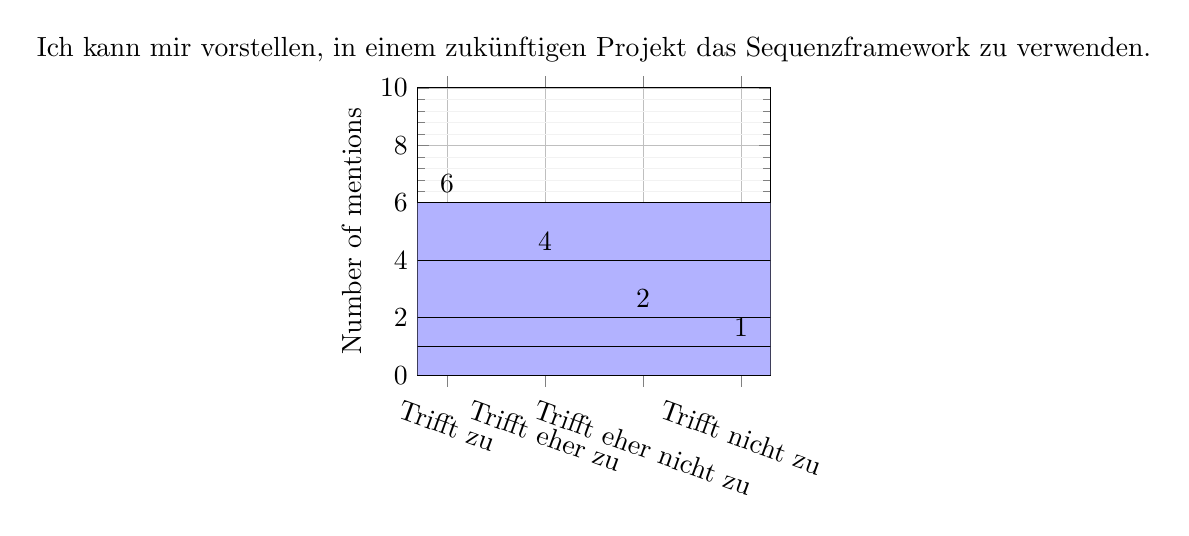
\begin{tikzpicture}
\begin{axis}[
% instead of scaling
width=\textwidth / 2, % Breite des Charts
title={Ich kann mir vorstellen, in einem zukünftigen Projekt das Sequenzframework zu verwenden.},
ybar,  % Art des Charts                                            
ymin=0, % y min
ymax=10, % y max
bar width=20, % Breite der Balken (in points)
nodes near coords, % Labels oberhalb der Bars
ylabel={Number of mentions},
grid=both, % Zeilen ds Grids
grid style={line width=.1pt, draw=gray!10},
major grid style={line width=.2pt,draw=gray!50},
minor y tick num=4,
xtick=data,
% use explicit ticklabels instead of symbolc x coords
xticklabels={Trifft zu, Trifft eher zu, Trifft eher nicht zu, Trifft nicht zu},
xticklabel style={ rotate=-20 },
]
\addplot[black,fill=blue!30!white]
coordinates{ (1,6) (2,4) (3,2) (4,1) };
\end{axis}
\end{tikzpicture}
\caption{Responses to "Ich kann mir vorstellen, in einem zukünftigen Projekt
das Sequenzframework zu verwenden."}
\label{fig:usertest_q1}
\end{figure}
% subsubsection Conclusion (end)
% subsection Findings Sequence library(end)
% section User Test Evaluation (end)
